% modernposter — A0 portrait, metropolis-inspired color scheme.
\documentclass{modernposter}

\title{A Legible Result Communicated Over Coffee}
\author{A. Researcher, B. Collaborator, C. Advisor}
\email{a.researcher@example.org}

\begin{document}
\maketitle

\begin{postercolumn}
	\posterbox{Introduction}{
		This poster is built on modernposter, a metropolis-inspired
		colour scheme laid over \texttt{a0poster}. Replace this box
		with the motivation for the work: the problem being solved,
		why it matters, and what gap the poster's result fills.
	}
	\posterbox{Methods}{
		\begin{itemize}
			\item Describe the approach, dataset, or apparatus here.
			\item A second bullet, for a second step of the method.
			\item A third, for whatever completes the picture.
		\end{itemize}
	}
	\posterbox{Result Figure}{
		\begin{center}
			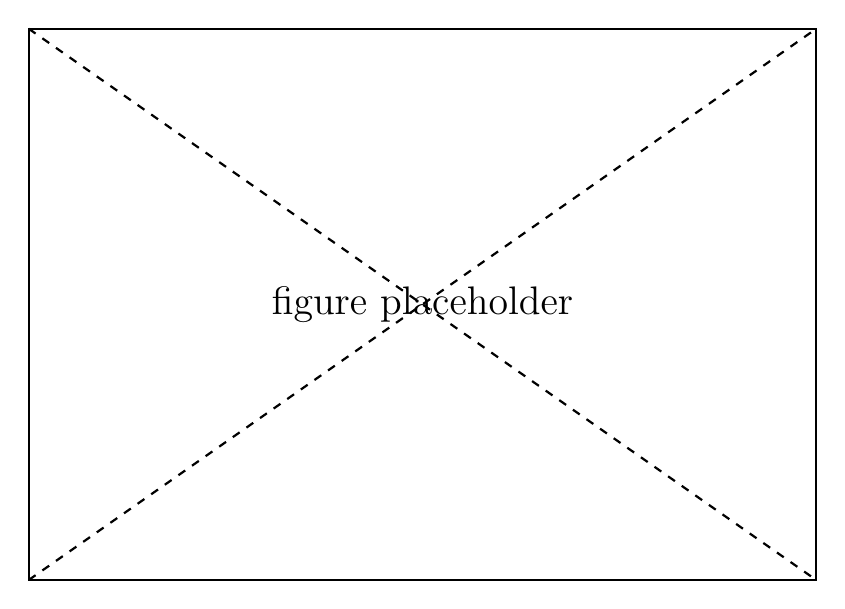
\begin{tikzpicture}
				\draw[thick] (0,0) rectangle (10,7);
				\draw[thick, dashed] (0,0) -- (10,7);
				\draw[thick, dashed] (0,7) -- (10,0);
				\node at (5,3.5) {\Large figure placeholder};
			\end{tikzpicture}
		\end{center}
	}
\end{postercolumn}

\begin{postercolumn}
	\posterbox{Result Table}{
		\centering
		\begin{tabular}{lcc}
			Condition & Metric A & Metric B \\
			\hline
			Baseline  & 0.42     & 12.3     \\
			Proposed  & 0.61     & 9.7
		\end{tabular}
	}
	\posterbox{Discussion}{
		Summarise what the result in the previous column means, and how
		it compares to prior work. This is also the natural place for
		limitations or threats to validity.
	}
	\posterbox{Conclusion}{
		One or two sentences stating the takeaway a passer-by should
		leave with, even if they read nothing else on the poster.
	}
	\posterbox{References}{
		[1] A. Author, ``A Foundational Paper,'' Journal of Examples,
		2020.

		[2] B. Author and C. Author, ``A Follow-up Study,'' Proc. of
		the Conference on Placeholders, 2022.
	}
\end{postercolumn}

\end{document}
